%%%%%%%%%%%%%%%%%%%%%%%%%%%%%%%%%%%%%%%%
%   Original by                                   %
% Athanassios Protopapas, October 2005 %
% Mini-example for using apa.cls       %
%                                      %
% modified by William Revelle, August, 2007 
%%%%%%%%%%%%%%%%%%%%%%%%%%%%%%%%%%%%%%%%

\documentclass[man]{apa}%can be jou (for journal), man (manuscript) or doc (document)
%
%
%these next packages extend the apa class to allow for including statistical and graphic commands
\usepackage{url}   %this allows us to cite URLs in the text
\usepackage{graphicx}  %allows for graphic to float when doing jou or doc style
\usepackage{amssymb}  %use formatting tools  for math symbols
% type setting of functions, packages, and R follows a particular style


\usepackage{multicol}
\usepackage{setspace}



\title{Are divergence point analyses suitable for response time data?}
\author{Pablo Gomez (1), Javier Breithaupt (2), Manuel Perea (2, 3), Jeff Rouder (4)}
\affiliation{(1) DePaul University, Chicago IL, USA \\ 
                 (2) Universitat de Val\`encia, Valencia, Spain \\ 
                 (3) BCBL, Basque Center on Cognition, Brain, and Language, San Sebasti\'an, Spain \\
                 (4) University of Missouri, Columbia MO, USA}
%taken from AP's user notes
% John Vokey uses something like this

\ifapamodeman{%

\note{\begin{flushleft}
Pablo Gomez\\
Department of Psychology\\
DePaul University\\
Chicago, Illinois\\
60614\\
e-mail: pgomez1@depaul.edu\\

   
\end{flushleft}}}


\abstract{
Estimating the time course of the influence of different factors in human performance is one of the principal topics of research in cognitive psychology/neuroscience. Over the past decades, researchers have proposed several methods to tackle this question using latency data. Here we examined a recently proposed procedure that employs survival analyses on latency data to provide ``precise estimates'' of the timing of the first discernible influence of a given factor on performance (e.g., word frequency on lexical access).  A number of articles have used this method in recent years, and hence an exploration of its strengths and its potential weaknesses is in order. Unfortunately our analysis revealed that the method has conceptual flaws, and it might lead researchers into believing that they are obtaining a measurement of a processing components when in fact they are obtaining a nonsensical measurement.
}

\acknowledgements{
The research reported in this article has been partially supported by Grant PSI2014-53444-P from the Spanish Ministry of Economy and Competitiveness. Pablo Gomez was the recipient of the \emph{Convitat} grant at the Universitat de V\`alencia.
}


\shorttitle{Survival and latencies}
\rightheader{Survival and latencies}
\leftheader{Gomez, Breithaupt, Perea \& Rouder}

\usepackage{Sweave}
\begin{document}
\Sconcordance{concordance:draftBRM.tex:draftBRM.Rnw:%
1 59 1 1 0 124 1 1 103 11 1}

\maketitle   



Perhaps the most common cognitive psychology experiment is one in which participants are presented with stimuli that vary in a dimension of theoretical interest (e.g., stimuli repetition, word frequency, etc.). The stimulus elicits a response, and researchers  measure latencies to make inferences about hypothesized underlying cognitive processes.  This form of mental chronometry is commonly used in the analyses of data from a broad range of experimental paradigms such as choice tasks, naming, eye-tracking, and many others.

   Although the most popular model of analysis are tests of mean latencies, the shortcomings of focusing only on  means to infer cognitive processes are well known (Balota \& Yap, 2011; Heathcote, Popiel, \& Mewhort, 1991; Ratcliff, 1979, Rouder, Lu, Speckman, Sun,  \& Jiang, 2005); indeed, theory development benefits from exploring distributional properties of latency measurements.  To take advantage of the distributional information of latency data, some researchers use methods that are based on fitting functional forms like the ex-Gaussian or the Weibull distributions (see Heathcote et al., 1991), while other researchers use methods that are based on process models like the diffusion model for choice response times (Ratcliff, 1978) or the EZ-reader model for eye fixation durations during reading (Reichle, Pollatsek, Fisher, \& Rayner, 1998). 
           
       There are several desired properties for any general method of analysis. These properties include (a) a method that uses distributional properties, (b) a lack of detailed assumptions about the underlying process, (c) a lack of specific assumptions the parametric form, (d) broad applicability in many paradigms, and (e) interpretability in theoretically meaningful terms. In this note, we explore a method, the \emph{divergence point analysis}, which is a procedure that seems to have all of  properties outlined above. The proponents of this method (Sheridan, 2013; see also Ando, Matsuki, Sheridan, \& Jared, 2015; Reingold \& Sheridan, 2014; Reingold, Reichle, Glaholt, \& Sheridan, 2012; Sheridan \& Reingold, 2013; Sheridan, Rayner, \& Reingold, 2013) aim to estimate the onset of the influence of a given variable on the basis of latency data; this onset is referred to as the \emph{divergence point}.
               
      Divergence point analysis utilizes survival functions in its estimation procedure; hence, a basic description of survival functions is helpful  Let $T$ be a random variable that denotes the response time and let $F(t)$ be its cumulative distribution function (CDF). The CDF denote the probability that the value of $T$ is smaller than some value $t$, i.e., $F(t)=Pr(T \leq t)$.  The survival function is the complement probability: $S(t)=Pr(T>t)=1-F(t)$, this is the probability that a response occurs later than some value t; hence at $t=0$, $S(0) = 1$ and at $t=\infty$, $S( \infty ) = 0$. There have been previous attempts to use survival functions in latency analyses.  Notably, Van Zandt (2002) examined several of these procedures and concluded that serious analyses of this type, ``would use samples of at least a few hundred observations" (p. 482). Along similar lines, Houpt and Townsend (2010, 2011) discussed a rather sophisticated method of survival analysis that involves experimental methods and a non-trivial algorithm termed survivor interaction contrasts.

       One of the appeals of the divergence point method is that it might overcome the limitations of traditional survival function analyses by using a computationally intensive bootstrapping procedure.  The divergent point method is a computational approach to assess when two survivor functions first diverge.  Each survivor function represents an experimental condition, say generically, experimental and control.  Processing is thought to be unaffected by the manipulation before the divergent time point and affected thereafter.  The time point then is the time in processing where the manipulation first has influence.  Understanding how these divergent time points depend on manipulations then provides a valuable insight into processing.

An example from Sheridan (2013) is provided in Figure 1.  The top panel shows vincentized latency distributions for first fixations and the goal is to assess the earliest point these distributions differ.  The corresponding survivor functions are shown in the bottom panel.  The thick horizontal bar shows time points where the survival functions differ significantly as determined by a bootstrap test.  The earliest such point, the vertical line, is the divergent point.  It the earliest point where the manipulation is said to start to affect processing.

       
       
       %The basic setup in the \emph{divergence point} method under consideration in this article can be described as follows: There are 10,000 iterations; in each iteration ($i^{th}$ iteration) the latencies for each participant and condition are randomly re-sampled with replacement. These sampled (bootstrapped) latencies are used to compute a survival curve for each participant,  which in turn are averaged across participants \emph{\`a la} Vincentile (Vincent, 1912). Next, for each time bin $t$ the difference between conditions: $\Delta_{t,i}$ is computed.  The final step is to sort, for each time $t$ the 10,000 $\Delta_{t,i}$'s.  The range between the $5^{th}$ and the $9,995^{th}$ value becomes the confidence interval $CI(\Delta t)$ and the divergence point is defined as the shortest $t$ at which the $CI(\Delta t)$ does not include 0. Aiming for a high temporal resolution, Sheridan and Reingold use $1 ms$ bins (see Figure~\ref{sheridan} for an example).%\footnote{We should note that in a recent paper, Reingold and Sheridan (2014) proposed some changes on the original version of the procedure by using confidence intervals rather than point estimates, but the both the conceptual and the technical limitations outlined in the present note apply equally to the original and the modified versions of the procedure.}.
      
\begin{figure}[h] %  figure placement: here, top, bottom, or page
	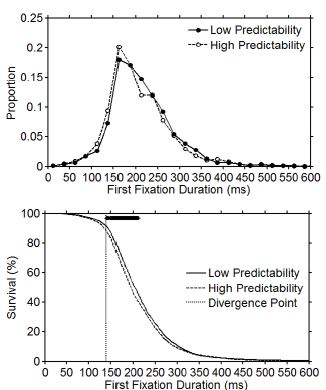
\includegraphics[width=3in]{Figure1.jpg}
	\caption{The figure (taken from Sheridan, 2013, p. 27) shows the distributions of first-fixation duration on target words in the low and high predictability conditions in the top panel, and the survival curves in the bottom panel. The row of points at the top of the survival curves indicates the time bins with a significant difference between the low and high predictability curves using the method being examined in the present note}
	    	\label{sheridan}
\end{figure}		

      Although this method might seem  promising and useful for researchers interested in exploring the time course of a given  empirical effect, there is a fundamental conceptual flaw in the foundation of the method.

\section{Estimating divergence points in latency distributions is conceptually flawed}

The \emph{divergence point} analysis rests on the notion that processing in two conditions proceeds in the same way until a point in time  (i.e., the divergence point). To show that this claim is flawed, we considered perhaps the simplest case.  Suppose processing was mediated by two stages which operated in serial manner.  The finishing time of the first stage is a normal with mean $\mu$ and standard deviation $\sigma$; the finishing time of the second stage is an exponential with scale $\tau$ (the latencies would follow an exgaussian distribution).  The manipulation of interest is assumed to affect only the later exponential stage, and it corresponds to a lengthening of scale $\tau$ for one of the conditions.   In this setup a divergence point might be expected, perhaps at $\mu$.  Figure~\ref{fig:x} shows the density function (PDF), the cummulative density (CDF), and survival functions for a hypothetical control and experimental conditions under these assumptions.  Perhaps counter intuitively, the CDFs have no common points to diverge from.  Instead, the distribution with the smaller exponential scale is faster everywhere. Obviously, if the manipulation of interest was in the the mean $\mu$ of the first stage the same conclusion holds as shown in Figure~\ref{fig:mu}. In both cases, the relationship is one of strict stochastic dominance.   If one is to talk about a divergence point at all, it would be at  $-\infty.$



\begin{figure}[h] %  figure placement: here, top, bottom, or page
	\includegraphics[width=5in]{xfig.pdf}
	\caption{The figure shows the density, cumulative density function and survival function of two distributions. The difference between the two distributions (the simulated effect) is in the rate ($\tau$) parameter of exponential component.}
		\label{fig:x}
\end{figure}



\begin{figure}[h] %  figure placement: here, top, bottom, or page
	\includegraphics[width=5in]{x2mu.pdf}
	\caption{The figure shows the density, cumulative density function and survival function of two distributions. The difference between the two distributions (the simulated effect) is in the rate ($\mu$) parameter of Gaussian component.}
		\label{fig:mu}
\end{figure}

This flaw in divergence point analyses is easy to understand as an error in logic.  The claim is based on a moment-to-moment view of processing on a single trial.  Yet, latency distributions are the collection of several trials in which latencies of eye movements latencies or key presses (for example) are collected. The properties of the distribution do not reflect the properties of any one specific trial.  The flaw is an example of distortions from aggregation which has been well known since Estes (1956).   As an exercise, we generated distributions with a true divergence point (525 ms) and realized that we needed to utilize a somewhat contrived procedure to generate these distributions: we assumed that latencies under 525 ms in one of the conditions would be substituted by a random number from an exponential distribution with scale = 121 to which we added a constant of 525; these distributions are shown in Figure~\ref{fig:contrived}. We then attempted to think of processing architectures that could yield a true divergence point of this type.  We considered diffusion models, counter models, race models, additive factor and stage insertion models.  These models all fail to produce a true divergence point.  In all cases, there is stochastic dominance, meaning that the divergence happens at the bottom or minimum of the distributions.  

After examining the architectures mention above, we were able to specify one case with true divergence: a mixture model where the components do not overlap at all.  Such a model is highly artificial and unrealistic in any setting.  It remains an open challenge, one that we suspect cannot be met, to find a plausible process model that predicts a non-minima divergence point. This is an important point, because without plausible mechanism to give rise to true divergence points, the numerical output of the method examine here is difficult to interpret.



\begin{figure}[h] %  figure placement: here, top, bottom, or page
	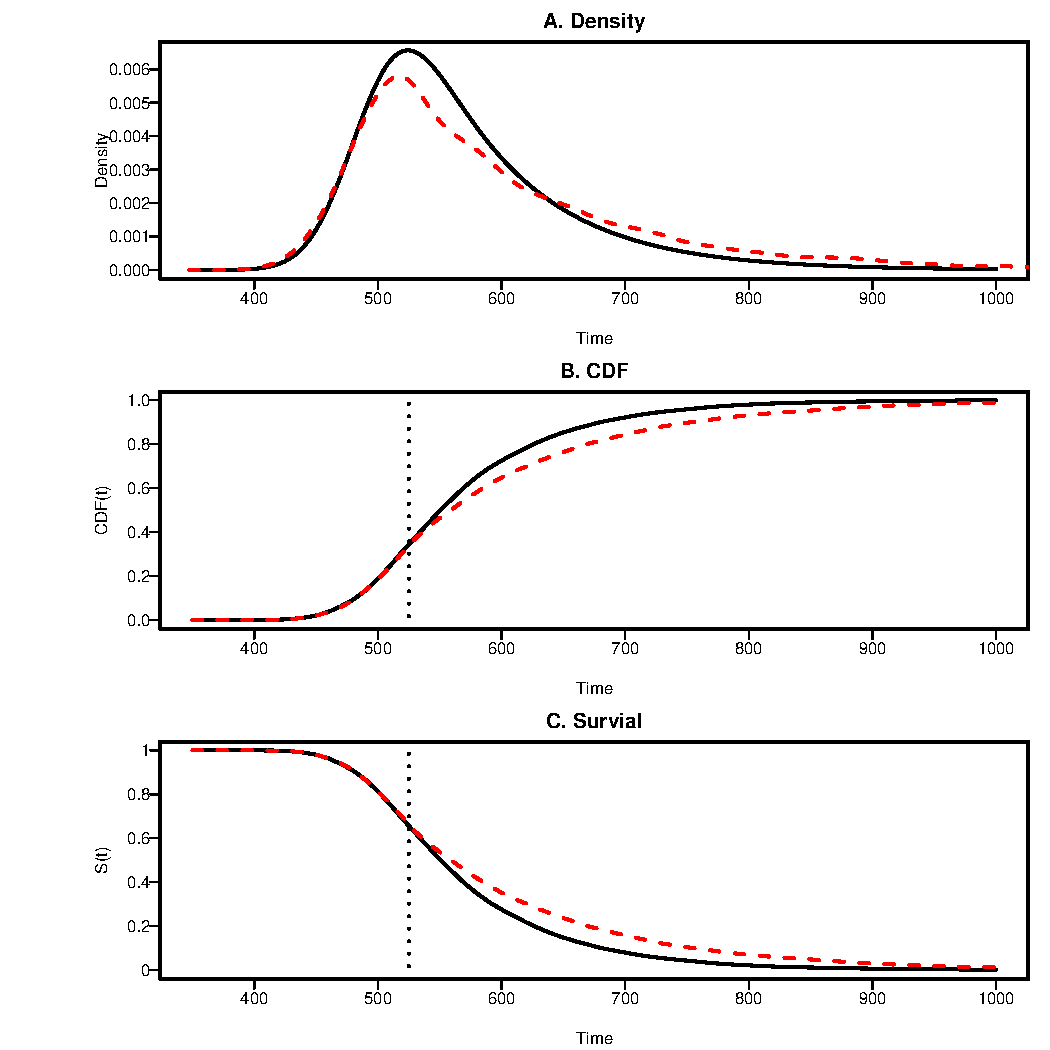
\includegraphics[width=5in]{contrived.pdf}
	\caption{The figure shows the density, cumulative density function and survival function of two distributions in which there is a divergence point (525 ms; the location of the vertical lines in Panels B and C)}
		\label{fig:contrived}
\end{figure}
  


 
            
  
\section{Conclusion}

Although the goals of the divergence point method are worth pursuing, our analysis revealed serious shortcomings on the conceptual foundation of the procedure:  Latency measurements tend to exhibit stochastic dominance between experimental conditions, and hence the divergence point would be at the leading edge of the latency distribution regardless of other distributional differences.  Furthermore, if the method is applied to data, an estimate of the divergence point will be provided by the method. This estimate will be affected mostly by the number of observations. In short, our exploration of the method forces us to conclude that in order to use the method, researchers should be sure that the latency distribution from their study indeed is produced by a process that yields identical PDF until a specific point in time. 

\newpage

\section{References}

Ando, E., Matsuki, K., Sheridan, H., \& Jared, D. (2015). The locus of Katakana-English masked phonological priming effects. \emph{Bilingualism: Language and Cognition, 18,} 101-117. doi: 10.1017/S1366728914000121


Balota, D. A., \& Yap, M. J. (2011). Moving beyond the mean in studies of mental chronometry the power of response time distributional analyses. \emph{Current Directions in Psychological Science, 20,} 160-166. doi: 10.1177/0963721411408885.


%Carreiras, M., Armstrong, B.C., Perea, M. \& Frost, R. , ( 2014 ). The What, When, Where, and How of Visual Word Recognition. \emph{Trends in Cognitive Sciences, 18,} 90-98.

Estes, W. (1956). The problem of inference from curves based on group data. \emph{Psychological Bulletin, 52}, 134-140. doi: 10.1037/h0045156.


Heathcote, A., Popiel, S. J., \& Mewhort, D. J. (1991). Analysis of response time distributions: An example using the Stroop task. \emph{Psychological Bulletin, 109,} 340-347. doi: 10.1037/0033-2909.109.2.340


%Heathcote, A., Brown, S., Wagenmakers, E. J., \& Eidels, A. (2010). Distribution-free tests of stochastic dominance for small samples. \emph{Journal of Mathematical Psychology, 54,} 454-463. doi: 10.1016/j.jmp.2010.06.005

Ratcliff, R. (1978). A theory of memory retrieval. \emph{Psychological Review, 85,} 59-108. doi: 10.1037/0033-295X.85.2.59 

Ratcliff, R. (1979). Group reaction time distributions and an analysis of distribution statistics. \emph{Psychological Bulletin, 86,} 446-461. doi: 10.1037/0033-2909.86.3.446

Reichle, E. D., Pollatsek, A., Fisher, D. L., \& Rayner, K. (1998). Toward a model of eye movement control in reading. \emph{Psychological Review, 105,} 125 -157. doi: 10.1037/0033-295x.105.1.125

Reingold, E. M., Reichle, E. D., Glaholt, M. G., \& Sheridan, H. (2012). Direct lexical control of eye movements in reading: Evidence from a survival analysis of fixation durations. \emph{Cognitive Psychology, 65,} 177-206. doi: 10.1016/j.cogpsych.2012.03.001 


Reingold, E. M., \& Sheridan, H. (2014). Estimating the divergence point: a novel distributional analysis procedure for determining the onset of the influence of experimental variables. \emph{Frontiers in Psychology, 5,} 1432. doi:10.3389/fpsyg.2014.01432

Rouder, J. N., Lu, J., Speckman, P., Sun, D., \& Jiang, Y. (2005). A hierarchical model for estimating response time distributions. \emph{Psychonomic Bulletin \& Review, 12,} 195-223. doi:10.3758/BF03257252

Sheridan, H. (2013). The Time-course of Lexical Influences on Fixation Durations during Reading: Evidence from Distributional Analyses. Doctoral Dissertation, University of Toronto. Retrieved from {\texttt https://tspace.library.utoronto.ca/bitstream/1807/35996/6/Sheridan\_Heathe\_201306\_PhD\_thesis.pdf}

Sheridan, H., \& Reingold, E. M. (2013). Distinct stages of word identification during reading: Evidence from eye movements. \emph{Journal of Vision, 13,} 511-511. doi:10.1167/13.9.511

Sheridan, H., Rayner, K., \& Reingold, E. M. (2013). Unsegmented text delays word identification: Evidence from a survival analysis of fixation durations. \emph{Visual Cognition, 21,} 38-60. doi:10.1080/13506285.2013.767296

Houpt, J. W., \& Townsend J. T. (2010). The statistical properties of the survivor interaction contrast. \emph{Journal of Mathematical Psychology, 54,} 446-453. doi:10.1016/j.jmp.2010.06.006

Houpt, J. W., \&. Townsend, J. T. (2011). An extension of SIC predictions to the Wiener coactive model, \emph{Journal of Mathematical Psychology, 55,}  267-270. doi:dx.doi.org/10.1016/j.jmp.2011.02.002.


Van Zandt, T. (2002). Analysis of response time distributions. In J. T. Wixted (Ed.), \emph{Stevens' Handbook of Experimental Psychology} (3rd ed., pp. 461-516). San Diego, CA: Academic Press. 


Vincent, S. B. (1912). The function of vibrissae in the behavior of the white rat. \emph{Behavioral Monographs, 1} (Whole No. 5).


\bibliography{bibfile-LDT}








\end{document}






